\chapter{BPMs System description}
In this section I describe the beam position monitor (BPM) system installed at the IP region and the signal analysis method used to test the system.\par
\section{The system}
The system consists in three cavities inside a vacuum chamber shown in Fig. \ref{f:vacuumchamberdes} which is fixed to the optical table used for the IPBSM laser and optical instruments. Flanges and viewports on the sides are compatible with the IPBSM operation. Inside the chamber, a system of three cavities (IPA, IPB and IPC) are installed in two separated blocks: one block upstream for IPA and IPB and the other downstream of the IP for IPC.\par
Each block is placed on top of a piezo-electric displacement system shown in Fig. \ref{f:piezosystem} with three degrees of freedom: vertical displacement, horizontal displacement and pitch angle. Position and angle conventions can be seen in Annex \ref{s:BPMscoord}. \par
\begin{figure}[htb]
\centering
\begin{subfigure}{0.4\textwidth}
 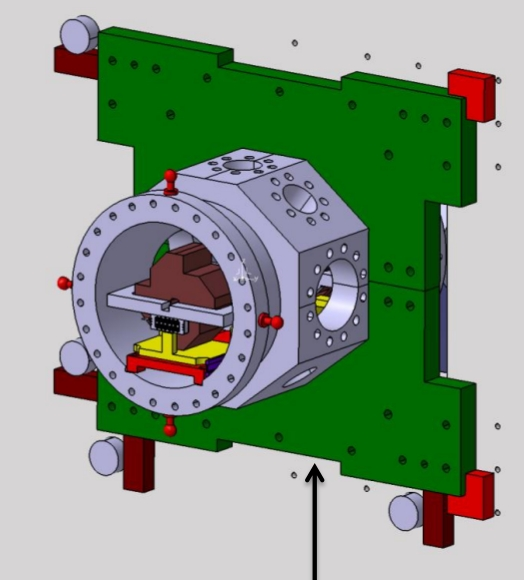
\includegraphics[scale=0.28]{chambrevide.jpg}\caption{Vacuum chamber design.}\label{f:vacuumchamberdes}
\end{subfigure}
\begin{subfigure}{0.5\textwidth}
 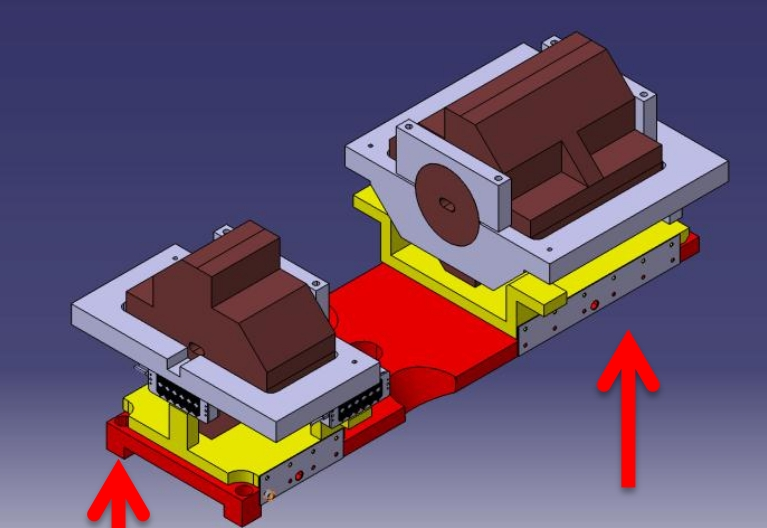
\includegraphics[scale=0.3]{BPMs01.jpg}\caption{Piezo-electric displacement system and cavities.}\label{f:piezosystem}
\end{subfigure}
\end{figure}
This piezo mover system is remotely controlled to align the cavities with the beam, and to do systematic studies of the cavity sensitivity to position change. A set of in-vacuum PT100 thermal gauges are included on each block. The initial checks on the system can be consulted in \cite{Bambade2013}, and the control and readout scheme can be seen in Annex \ref{s:annexB} with alignment results.\par
\subsection{The cavities}
Cavities for beam position measurement must have good stability since precision depends on mechanical precision. Resolution at thermal noise level of the readout electronics can be achieved by narrowing the dynamic range and using high gain electronics since signal is small near the cavity center. The following is a description of the cavity parameters as presented by Nakamura in \cite{Nakathese}.\par
\subsubsection{Cavity modes}
The cavity consists of a cavity and a waveguide. When the particles passes through the cavity, it resonates in several modes at frequencies given by the cavity dimension and shape \cite{PhysRevSTAB.15.042801}.\par 
Cylindrical coordinates are used for cylindrical cavities. The electric $E=(E_r,E_\phi,E_z)$ and magnetic field $B=(B_r,B_\phi,B_z)$ are excited in the cavity. For beam position monitoring the transverse mode (TM) $B=(B_r,B_\phi,0)$ is essential. Three numbers $m,n,l$ which are the mode numbers in $r,\phi,z$ are used to identify the modes. The TM$_{010}$ is the monopole mode and it is used for charge intensity measurement and downmixing of the signals from the position sensitive cavities. It is shown in Fig. \ref{f:monopole}.\par
In a similar way, rectangular coordinates are used for rectangular cavities. The electric $E=(E_x,E_y,E_z)$ and magnetic field $B=(B_x,B_y,B_z)$ are excited in the cavity. For beam position monitoring the TM $B=(B_x,B_y,0)$ is essential. Three numbers $m,n,l$ which are the node numbers in $x,y,z$ are used to identify the modes. The TM$_{120}$ and TM$_{210}$ are the dipole modes and are used for bunch position measurement. The TM$_{110}$ is the monopole mode in rectangular cavities. They are shown in Fig. \ref{f:dipole}.\par
\begin{figure}[htb]
\centering
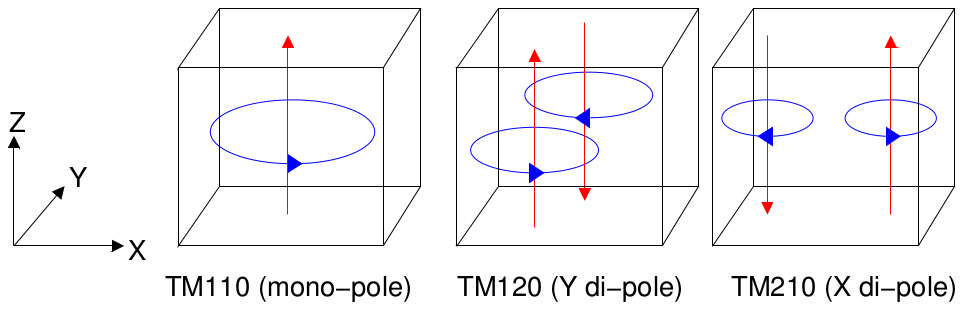
\includegraphics[scale=0.4]{TMdipole.jpg}.\caption{Dipolar and monopolar mode in rectangular cavities.}\label{f:dipole}
\end{figure}
\begin{figure}[htb]
\centering
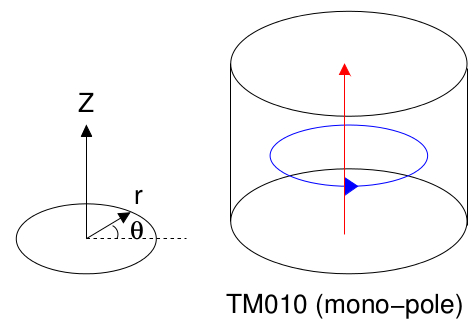
\includegraphics[scale=0.4]{TMmonopole.jpg}.\caption{Monopolar mode in cylindrical cavities.}\label{f:monopole}
\end{figure}
Only the dipole mode is of interest for beam position measurement so it is separated from other modes which are considered noise components. The separation between the vertical and horizontal dipole mode is made by making the cavity rectangular, resulting in different resonant frequencies for each plane.\par
A set of slots is introduced on the cavity walls to couple only the dipole mode to a waveguide with a cut-off frequency above the monopole mode. This is made to separated the dipole signal from large noise coming from the monopole component. An antenna picks up the signal in the waveguide and connects it to the output port. The cavity design has then four ports, two ports in antiphase per plane, one on each side. Figure \ref{f:waveguide} shows the cavity transversal plane with the four slots and the coupling to the waveguide and antena for the horizontal ports.\par
\begin{figure}[htb]
\centering
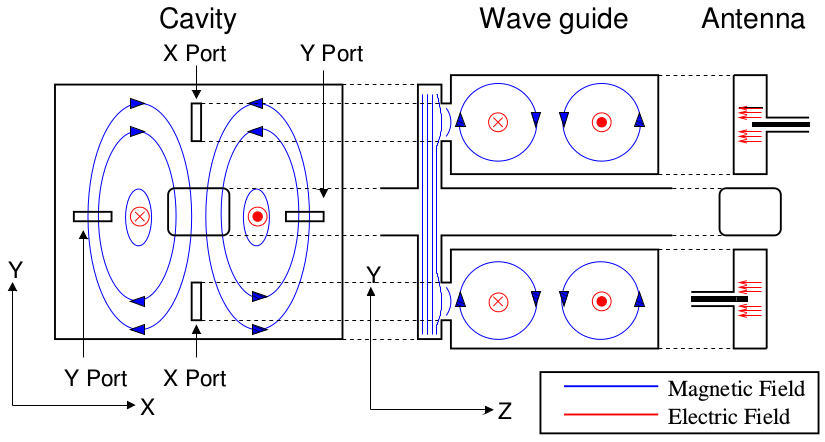
\includegraphics[scale=0.4]{Waveguide.jpg}.\caption{Coupling to the dipole mode of the cavity.}\label{f:waveguide}
\end{figure}
\subsubsection{Output signal}
Voltage of a resonant mode excited in a cavity by a passing beam, $V_{exc}$, is expressed as
\begin{equation}
 V_{exc}=\frac{\omega}{2}\left(\frac{R}{Q}\right)q
\end{equation}
where $\omega$ is the resonant angular frequency of the mode, $q$ is the beam charge, $R$ is the shunt impedance and $Q$ is the quality factor which represents the efficiency of the resonant mode of a cavity. The factor $R/Q$ is
\begin{equation}
 \frac{R}{Q}=\frac{|\int E\cdot ds|^2}{\omega U}
\end{equation}
where $U$ is the energy stored in the cavity and $E\cdot ds$ is the longitudinal component of the electric field in the cavity generated by the passing beam. The cavity design for the IP region targets high $R/Q$ (high $Q_0$), minimizing the energy loss in the cavity walls and maximizing the output power.\par
The finite bunch length $\sigma_z$ results in an effective reduction of $V_{exc}$ given by the expression
\begin{equation}
 V_{totalexc}=V_{exc}\exp\left(-\frac{\omega^2\sigma_z^2}{c^2}\right)
\end{equation}
The stored energy of a cavity is $U=V_{totalexc}^2/(\omega R/Q)$, and the output power is $P_o=\omega U/Q_{ext}$, where $Q_{ext}$ is the quality factor of the external coupling. Detecting the power output, $P_o$, by an impedance $Z$ gives the output voltage
\begin{equation}
 V_{out0}=\sqrt{ZP_{o}}=\frac{wq}{2}\sqrt{\frac{Z}{Q_{ext}}\frac{R}{Q}}\exp\left(-\frac{\omega^2\sigma_z^2}{2c^2}\right)
\end{equation}
% \subsubsection{Decay time}
The energy dissipation in the cavity is
\begin{equation}
 U=U_0 e^{-\frac{\omega}{Q_L}t}
\end{equation}
where $\frac{1}{Q_L}=\frac{1}{Q_0}+\frac{1}{Q_{ext}}$, and the energy decay time $\tau=Q_L/\omega$. As the signal is proportional to the square root of the power, then the signal decay time is a factor two smaller.\par
Finally, as the $R/Q$ factor depends on the longitudinal component of the electric field, the integration depends on the TM mode. It has been derived in \cite{Nakathese} concluding that in the dipole mode $R/Q$ depends on the square of the bunch transverse position in the case of bunches passing near the center, while the monopole mode $R/Q$ is independent of position. From this, the output voltage in the TM$_{120}$ and TM$_{210}$ is proportional to position, while TM$_{110}$ and TM$_{010}$ are not.\par
\subsubsection{Components orthogonal to position}
Additional components are present in the cavity signal output which are orthogonal to bunch position. They have been described in \cite{Nakathese} as
\begin{equation}
 V=V_{position}+iV_{angle}+iV_{pitch}+iV_{commontail}
\end{equation}
where the imaginary factor $i$ involves a $\pi/2$ phase difference, and the following is a brief description of each component:\par
\begin{itemize}
 \item Angle: a cavity of length $L$ gives a position voltage as $V_{position}=Ax\sqrt{L}\sin(\omega t)$. Assuming a beam passing through the cavity center making an angle $x'$, it can be decomposed as the sum of two position signals with $x=x'L/4$ and phase difference of $\pm L/4c$, affecting the amplitude by $\sin(\omega L/4c)$ and the phase by $\pi/2$. The ratio of angle to position signals for $\omega L/4c\ll 1$ is
 \begin{equation}
  \frac{|V_{angle}|}{|V_{pos}|}=\frac{\omega L^2}{2\sqrt{2}c}\frac{x'}{x}
 \end{equation}
\item Pitch: a cavity gives a position voltage as $V_{position}=Aqx\sin(\omega t)$. The beam is decomposed in two points with $q/2$ total charge each, while traversing the cavity with an angle $\theta$. The sum of two position signals with $q/2$ charge each,  $x=\sigma_z\theta$ being $\sigma_z$ the bunch charge, and phase difference of $\pm\sigma_z/c$ will affect the amplitude by $\theta\sigma_z^2/c$ and the phase by $\pi/2$. The ratio of angle to position signals is
\begin{equation}
  \frac{|V_{pitch}|}{|V_{pos}|}=\frac{\omega \sigma_z^2}{c}\frac{\theta}{x}
\end{equation}
\item Commontail: the common-tail \cite{Shintake:1998fga} comes from the monopole component. At the dipole component frequency it is 2 to 3 orders of magnitude stronger that the dipole component. However, it is attenuated by the coupling to the waveguide. Nakamura \cite{Nakathese} shows that the phase advance between the monopole and the dipole signals is $\pi/2$.\par
\end{itemize}
The phase difference of these components allows one to remove them from the position signal by phase detection. In addition the cavity design was conceived to reduce the angle signal by making it short to mitigate the effects from the large beam divergence seen in Section \ref{s:opticsIP}.\par
\subsubsection{Cavities at the IP Region}\label{s:IPBPMsignals}
The three cavities (IPA, IPB and IPC) are rectangular and resonate in the TM$_{210}$ and TM$_{120}$ modes, at the C-band frequency of 5.7 and 6.4~GHz, in the horizontal and vertical planes, respectively. They have a design decay time of 19~ns (horizontal) and 17~ns (vertical), and sensitivities to bunch position of 2.2~$\mu$V/nm/nC (horizontal) and 3.7~$\mu$V/nm/nC (vertical). Two additional cylindrical cavities with decay time of 29~ns, sensitivity to bunch charge of 3.27~V/nC, one per resonant frequency, are placed downstream of the IP to measure the bunch charge and to enable downmixing the C-Band frequency signals in the readout (see Section \ref{s:processing}); these are the reference cavities.\par
The IPA, IPB and IPC sensitivity to orthogonal components are: position to angle ratio of 3.2~$\mu$m/mrad, position to bunch pitch ratio of 8.6~$\mu$m/mrad with $\sigma_z$=8~mm and unknown commontail component.\par
Previous to the installation, the cavity signals' decay time was measured giving the results shown in Table \ref{t:decayt}. In particular IPC shows a shorter decay time than IPA and IPB. The effect of the large difference between the design and the measured values on resolution is currently under investigation.\par
\begin{table}[h]
\centering
\begin{tabular}{c|c||c|c|c}\hline
 Plane & Design & IPA & IPB & IPC \\\hline\hline
  X [ns] & 19.41 & 8.722 & 8.181 & 4.925\\
  Y [ns] & 17.49 & 11.11 & 11.25 & 6.745\\\hline
\end{tabular}\caption{Measured decay time for the three cavities before installation.}\label{t:decayt}
\end{table}
The reference cavities have been tuned to match the measured resonant dipole frequency from the sensor cavities, showing maximum difference of 3.5~MHz in Table~\ref{t:dipolefreq}, and good agreement with the design. 
\begin{table}[h]
\centering
\begin{tabular}{c|c||c|c|c|c}\hline
 Plane & Reference & Average & IPA & IPB & IPC \\\hline\hline
  X [MHz] & 5712 & 5712 & -2 & -2.5 & +2.5\\
  Y [MHz] & 6426 & 6420 & +1 & 0 & -3.5\\\hline
\end{tabular}\caption{Resonant dipole frequency measurement at KEK before installation.}\label{t:dipolefreq}
\end{table}

\subsection{The processing electronics}\label{s:processing}
Each position measurement cavity has two output ports in antiphase per plane connected to independent processing electronics  to downmix the signals, separate them into two orthogonal components called $I$ and $Q$, and set the gain according to beam charge conditions. A set of remotely-controllable attenuators, variable between 0-70 dB in steps of 10 dB can be used to increase the linear range of electronics at the expense of resolution.\par
At the moment the reference cavities are not used to downmix the position cavities signals directly to base band. Instead, as explained below, a 714~MHz signal from the DR is used to downmix the three cavity signals to 714~MHz in a first stage and then a second stage downmixes the position cavities to baseband using the reference cavity signal. This allows the installation of the second stage outside the ATF2 line, aiming at studying the signals with different phase detection settings changed by hand in the hardware. An scheme of the electronics is shown in Fig.~\ref{f:elect}. The following is a description of components extracted from \cite{Nakathese}.\par
\begin{figure}[htb]
 \centering\hspace*{-1cm}
 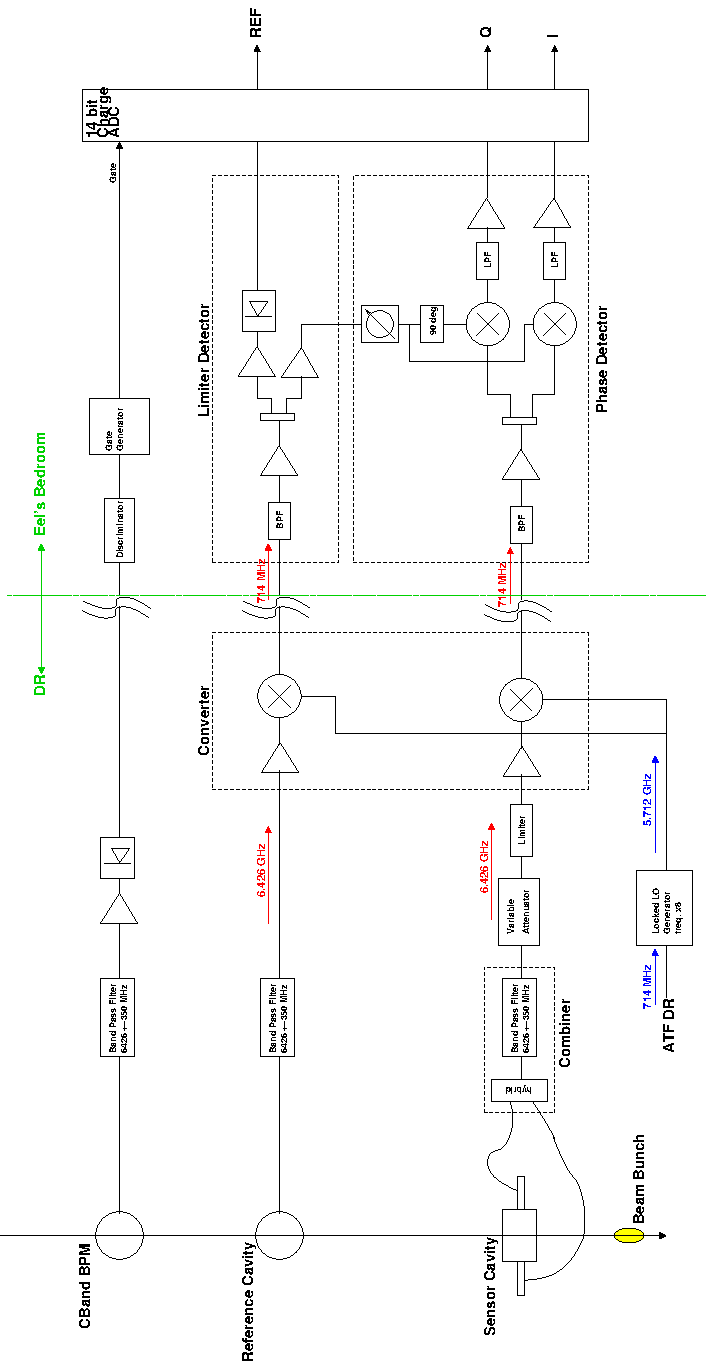
\includegraphics[scale=0.7,angle=-90]{Electr-crop.pdf}\caption{Processing electronics per BPM per plane.}\label{f:elect}
\end{figure}
\begin{itemize}
 \item Combiner: The combiner outputs the difference of the signals. However, the signal from the two cavity ports are in antiphase so the net effect is factor 2 of amplification.\par
 \item Variable attenuator: it attenuates the input signal from 0~dB to 70~dB in steps of 10~dB. The purpose is to enlarge the dynamic range at the expense of resolution.\par
 \item First stage of down conversion: it downmixes the BPM and reference cavity signals to 714~MHz using an $8\times714$~MHz (for the vertical plane) and $9\times714$~MHz (for the horizontal plane) signal from the LOCKED LO module, and amplifies the output by 20~dB. It is required to do it as close as possible to the BPMs because of the short decay time.\par
 \item LOCKED LO: Multiplies the frequency of the DR 714~MHz by a factor 8 for the vertical plane and 9 for the horizontal plane to perform the first stage of signal downmixing.\par
 \item Limiter detector: Set a constant amplitude of the Reference signal at 714~MHz to be used for the downmixing in the second stage. Fig. \ref{f:detector} shows a diagram with 4 outputs to be used for downmixing. It also outputs the signal proportional to charge.\par
 \item Phase detector: It sets the common phase between the ref cavity signal and the IPBPMs signals by means of a knob. Then, it separates the IPBPMs signals in two set of orthogonal components by downmixing the signals at 0\textdegree, 90\textdegree, 45\textdegree and 135\textdegree. The outputs at 0\textdegree and 90\textdegree are amplified by 25 to 30~dB, and the 45\textdegree and 135\textdegree outputs by extra 10~dB acording to the module used. One of the two orthogonal sets is read out as In-phase ($I$) and Quadrature-phase ($Q$).\par
\end{itemize}
\begin{figure}[htb]
 \centering%\hspace*{-1cm}
 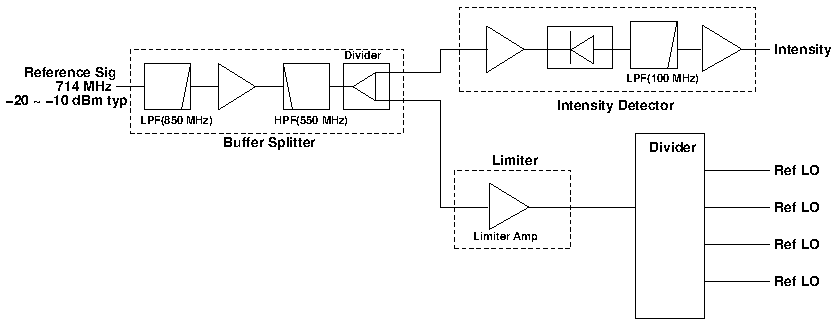
\includegraphics[scale=1.0,angle=0]{Detector-crop.pdf}\caption{Limiter detector.}\label{f:detector}
\end{figure}
At the moment only one Limiter detector is available, therefore, acquisition of only four signals was possible. Priority was given to the study of the three IPBPMs vertical signals. The horizontal signals were studied only for alignment matters.\par
The noise floor of the first stage of downmixing has been previously measured to be -95~dBm (4~$\mu$V$_{rms}$). It limits the resolution to 2~to~3~nm (horizontal) and 1~to~2~nm (vertical) at $0.5\times10^{10}$ particles per bunch because of sensitivities shown in Sect. \ref{s:IPBPMsignals}.\par
The gain and attenuation settings are used to achieve the maximum dynamic range within the acquisition system limits described in Sect. \ref{s:acqsys}.
The dynamic range of the electronics is estimated as follows: at 10~dB attenuation, for $0.4\times10^{10}$ particles and 3.7~$\mu$C/nm/nC vertical position sensitivity the signal is 0.75$\mu$V/nm. This signal is amplified by a total of 53.7~dB from the first (+20~dB) and second (+43.7~dB) downmixing stages with 10~dB losses estimated from cables and couplers. Using +2.5~V as maximum range of acquisition, the signal dynamic range is 6.9~$\mu$m. This can be directly compared with the dynamic range measurement in Sect. \ref{s:dynrange}.\par
However, the typical input value to the first downmixing stage is of -60~dBm (223.7$\mu$V$_{rms}$). It results in a much tighter dynamic range of 300~nm. The estimated input signal to the first downmixing stage and 6.9~$\mu$m offset is only -33~dB (5~mV$_{rms}$).\par
\subsection{Feedback system}
A local beam-based feedback system has been installed at the IP, in order to stabilise the beam position at the IP. This system comprises a stripline kicker, just upstream of the IP chamber, a fast kicker amplifier and digital feedback controller, and can be driven by any of the three IPBPM $IQ$ signals, or a linear combination of the signals from any two BPMs. The system is designed for operation within bunch train of two or more bunches, separated by less than 150-200~ns, where the measurement of the first bunch provides the input to the feedback system, and the correction is applied to subsequent bunches.\par
\subsection{The acquisition system}\label{s:acqsys}
The acquisition system samples the two downmixed orthogonal waveforms per cavity per plane over the decay time. This amounts to 14 simultaneous channels: $I$ and $Q$ waveforms for both $x$ and $y$ for each of the three position measurement cavities plus the charge signal from each of the two reference cavities.\par
The resolution required to measure 1~nm over the 10~$\mu$m of dynamic range is at least 14 bits ($2^{14}$ discrete steps). However, several systems have been used during the course of the IPBPM operation.\par
Initially a set of four Agilent 3000 X-Series oscilloscopes of 8~bits resolution, four channels each, $5$V$_{rms}$ dynamic range and up to 4~Gsamples/s was used for IPBPMs commissioning. Also a dedicated acquisition board, FONT5, operated by FONT group to perform the IP feedback was used. It digitised 9 channels synchronized in banks of three, 13~bits resolution, and a maximum sampling of 400~MHz with $\pm$0.5~V dynamic range.\par
A dedicated acquisition system built around a SIS digitizer has recently been introduced. The resolution is 14-bits, the dynamic range is either 2 or 5~V, and the sampling frequency is configurable with 238~MHz being the typical value. This is an important step towards integration of the IP position measurements into the existing ATF control system because of the gain in dynamic range, higher resolution and assured data availability.\par
\section{BPM Analysis Method}
The system has been tested with three sets of optics : (1) parallel beam (large beam size at waist and hence approximately constant beam size through the IP region) (2) nominal and (3) low beta.\par
The longitudinal position of the beam focus was moved closer to the location of IPB, by changing the strength of the FD, to reduce the beam jitter at IPB, allowing operation without additional attenuation and hence maximal sensitivity.\par
\subsection{Waveform analysis}
The $I$ and $Q$ waveforms are analysed by choosing a single sample point on the signal. In general, the on-peak sample is chosen except in cases where the post analysis shows saturation of the processing electronics. The identification of position and orthogonal components requires a position scan, as explained in Section \ref{s:posscan}.\par
Averaging or integrating the samples may do something to improve the analysis due to the presence of $(714\pm10)$~MHz band pass filters between the first and second stage of downmixing of the processing electronics as part of an investigation into the reduction of large unwanted static waveform components.\par
\subsection{Position scans}\label{s:posscan}
While the beam is running the cavity position is systematically changed and the $I$ and $Q$ waveforms are acquired and analysed offline to obtain the signal change to displacement ratio, known as calibration factor.\par
By definition $I'$ is the position signal and $Q'$ contains all signals orthogonal to position. Figure~\ref{f:IQrot} shows that a systematic change in $I'$ signal could change the $I$ and $Q$ values because of a relative phase fixed by the detector in between the reference and the $IQ$ signals. In addition, the mismatch between the BPM dipole frequencies with respect to the reference cavity frequency generates a constant rotation of the $I$ and $Q$ signals which depends on the chosen sample on the waveform.\par
\begin{figure}[htb]
 \centering%\hspace*{-1cm}
 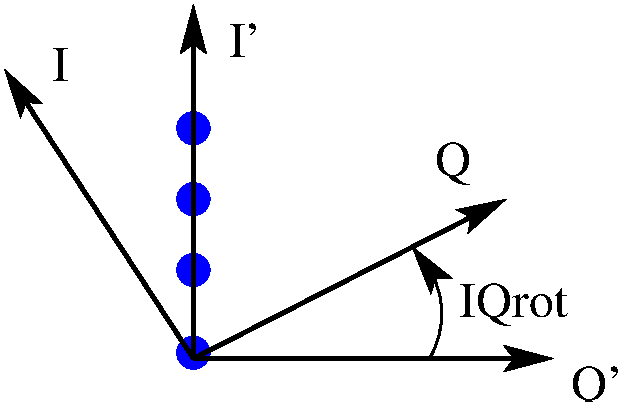
\includegraphics[scale=0.5,angle=0]{IQrot.pdf}\caption{IQ rotation. The blue dots represent the systematic change in position.}\label{f:IQrot}
\end{figure}
The position scan analysis allows to identify $I'$ and $Q'$ by the following procedure:
\begin{itemize}
 \item Single samples in the waveform for $I$, $Q$ and $Ref$ signals are chosen.\par
 \item The $I$ and $Q$ values per pulse are divided by the $Ref$ value, in order to remove the charge dependence. We have now $I_n$ and $Q_n$.\par
 \item Plotting $I_n$ vs $Q_n$ allows one to find the $IQ$ rotation angle, $IQ_{rot}$.\par
 \item The $I_n$ and $Q_n$ are counter rotated by the $IQ_{rot}$ angle, to determine $I'$ and $Q'$.
\end{itemize}
The ratio $I'/\Delta y$ in a.u./$\mu$m is the cavity calibration factor, $C_{bpm}$.\par
It also gives the information of the beam center position, $I'=0$, and the amplitud in $\mu$m of the constant orthogonal component $Q'/C_{bpm}$.\par
\subsection{Angle scans}
First a position scan should be done to identify $I'$ and $Q'$ signal. Then, a combination of piezo-movers setting keep the cavity center stable and changes the BPM pitch angle in systematic steps while the beam is running. See Appendix \ref{s:alignadj} for the required mover settings for angle scans.\par
The $I$ and $Q$ signals are analysed applying the $IQ_{rot}$ angle from the position scan, and it will show the change in $I'$ and $Q'$ while changing the angle. The $Q'/\theta_p$ and the calibration factor from the position scan are divided to find the angle to position ratio. It has been measured for IPBy giving 3.2~$\mu m$/mrad as expected from cavity parameters~\cite{Neven2014} (see Section \ref{s:IPBPMsignals}).\par
\subsection{Jitter acquisitions}
The beam jitter is determined from measurements of the bunch position over several hundred pulses with static BPM mover settings.\par
Consider now the signal $S$ as the sum of the two outputs from the cavity. The signal $S$ for the vertical outputs of one BPM and one bunch is composed of:
\begin{equation}
S = y+is_p\theta_p+s_{xy}(x+is_y\theta_y)+x\theta_r
\end{equation}
where $i$ represents the $\pi/2$ phase difference, $s_p$ is the sensitivity to pitch angle, $s_{xy}$ is the inverse of X-Y isolation, $s_y$ is the yaw angle sensitivity and $x,y,\theta_p,\theta_r,\theta_y$, are horizontal position, vertical position, pitch, roll and yaw angles of the BPM with respect to beam.\par
The signal $S$ can be separated in real and imaginary parts:
\begin{equation}
S = (y+s_{xy}x+x\theta_r)+i(s_p\theta_p+s_{xy}s_y\theta_y)
\end{equation}
The amplitude $|S|$ is the total contribution to signal and should be below the dynamic range of the first downmixing stage.\par
This signals are rotated by an arbitrary angle $\phi$ to obtain the $I'$ and $Q'$ at the phase shifter block.
\begin{align*}
S &= \underbrace{(y+s_{xy}x+x\theta_r)(\cos\phi+i\sin\phi)}+\underbrace{i(s_p\theta_p+s_{xy}s_y\theta_y)(\cos\phi+i\sin\phi)}\\
  &= I' + Q' 
\end{align*}
In the case of perfect IQ rotation ($\phi=0$), all the imaginary (angle and others) component is removed from the real (position) component in the $S$ signal. However, in practice this rotation could be achieved to a precision $\Delta\phi$, then, to first order
\begin{equation}
S=[(y+s_{xy}x+x\theta_r)-\Delta\phi(s_p\theta_p+s_{xy}s_y\theta_y)]+i[\Delta\phi(y+s_{xy}x+x\theta_r)+(s_p\theta_p+s_{xy}s_y\theta_y)]
\end{equation}
At this point we will only be interested in the real part as it contains most of the vertical position signal.
\begin{equation}
 \Re[S]=S_y = (y+s_{xy}x+x\theta_r)-\Delta\phi(s_p\theta_p+s_{xy}s_y\theta_y)
\end{equation}
The last equation shows the contribution to vertical signal from the relative position of the BPM to the beam.\par
The mean value of the $S_y$ signal over $m$ bunch samples will be equal to
\begin{equation}
 \langle S_y\rangle = [y_0+(x_0+\eta\delta)(s_{xy}+\theta_{r0})]-\Delta\phi[s_p\theta_{p0}+s_{xy}s_y(\theta_{y0}+\eta'\delta)]
\end{equation}
where all parameters 0-index correspond to misaligments, $\eta$ and $\eta'$ are the spatial dispersion and angular dispersion optical functions, $\delta=10^{-3}$ is the energy spread, and no beam rotation is considered. The alignment purpose is to make $\langle S\rangle =0$.\par
The variance of the signal jitter $\sigma_{S_y}^2=\langle S_y^2\rangle-\langle S_y\rangle^2$ can be expressed as\par
\begin{align*}
 \sigma_{S_y}^2=&\sigma_{jy}^2+\sigma_{jx}^2[s_{xy}+\theta_{r0}]^2+(\Delta\phi)^2[s_p^2\sigma_{jy'}^2+s_{xy}^2s_y^2\sigma_{jx'}^2]\\
 =&\langle y^2\rangle-y_0^2+(\langle x^2\rangle-x_0^2)[s_{xy}+\theta_{r0}]^2+(\Delta\phi)^2[s_p^2(\langle y'^2\rangle-y'^2_0 +s_{xy}^2s_y^2(\langle x'^2\rangle-x'^2_0)]
\end{align*}
and substracting all means effects
\begin{equation}
 \sigma_{S_y}^2=\langle y^2\rangle+\langle x^2\rangle[s_{xy}+\theta_{r0}]^2+(\Delta\phi)^2[s_p^2\langle y'^2\rangle+s_{xy}^2s_y^2(\langle x'^2\rangle)]
\end{equation}
Isolation X-Y (1/$s_{xy}$) was measured to be under 50dB% (Pin/Pout$<10^{-5}=3.162\times10^{-3}$ voltage isolation)
, sensitivity to pitch ($s_p$) was measured to be $3.2\mu$m/mrad, and sensitivity to yaw ($s_y$) is 2.9$\mu$m/mrad estimated in similar way as $s_p$.\par
For a 1~nm contribution to beam size we get:
\begin{align}
 1~\text{nm}\geq &\sqrt{\langle x^2\rangle}[s_{xy}+\theta_{r0}]&=&\sqrt{\langle x^2\rangle}[1.880\times10^{-3}+\theta_{r0}]\\
 1~\text{nm}\geq &\Delta\phi s_p\sqrt{\langle y'^2\rangle}&=& 3.2\Delta\phi\sqrt{\langle y'^2\rangle}\\
 1~\text{nm}\geq &\Delta\phi s_{xy}s_y\sqrt{\langle x'^2\rangle}&=&5.453\times10^{-3}\Delta\phi\sqrt{\langle x'^2\rangle}
\end{align}
where  the BPM vertical (3.7mV/$\mu$m/nC) and horizontal (2.2mV/$\mu$m/nC) sensitivities have been used to translate voltage isolation X-Y to position scale, position jitter is in nm and angle jitter in $\mu$rad.\par
Tables \ref{t-jitter1BX1BY}-\ref{t-jitter10BX1BY-IPA} show the typical jitter magnitude at the beam waist and the farthest BPM (IPA) for the two optics with the largest angular jitter.\par
Using the above jitter magnitudes at the beam waist for the 10BX1BY optics, one can calculate that $\theta_{r0}\leq 0.6$~
mrad and $|\Delta\phi|\leq 4.525$~mrad are required to 1~nm resolution.\par
The current precision of $|\Delta\phi|$ has been found to be 43~mrad by redoing 7 calibrations one after another. This is 10 times bigger than specified and could contribute to 3~to~4~nm to the position jitter at the IP because it adds up in quadrature.
% \pagebreak
\begin{table}[h]
\centering
 \begin{tabular}{|c|c|c|}\hline	
 Jitter &10\% & 20\%\\\hline
 $\sigma_{yj}$(nm) & 3  & 7\\\hline
 $\sigma_{xj}$(nm) &283&565 \\\hline
 $\sigma_{y'j}$($\mu$rad) &34&69\\\hline
 $\sigma_{x'j}$($\mu$rad) &71&141\\\hline
 \end{tabular}
 \caption{Jitter at beam waist with 1BX1BY optics.}\label{t-jitter1BX1BY}
\end{table}
\begin{table}[h]
\centering
 \begin{tabular}{|c|c|c|}\hline
 Jitter &10\% & 20\%\\\hline
 $\sigma_{yj}$(nm) & 3  & 7\\\hline
 $\sigma_{xj}$(nm) &894&1787 \\\hline
 $\sigma_{y'j}$($\mu$rad) &34&69\\\hline
 $\sigma_{x'j}$($\mu$rad) &22&44\\\hline
 \end{tabular}
 \caption{Jitter at beam waist with 10BX1BY optics.}\label{t-jitter10BX1BY}
\end{table}
\begin{table}[t]
\centering
 \begin{tabular}{|c|c|c|}\hline
 Jitter &10\% & 20\%\\\hline
 $\sigma_{yj}$(nm) & 5766  &11531\\\hline
 $\sigma_{xj}$(nm) &11866&23733 \\\hline
 $\sigma_{y'j}$($\mu$rad) &0&0\\\hline
 $\sigma_{x'j}$($\mu$rad) &1&3\\\hline
 \end{tabular}
 \caption{Jitter at IP with 1BX1BY optics.}\label{t-jitter1BX1BY-IPA}
\end{table}
\begin{table}[t]
\centering
 \begin{tabular}{|c|c|c|}\hline
 Jitter &10\% & 20\%\\\hline
 $\sigma_{yj}$(nm) &5766&11531\\\hline
 $\sigma_{xj}$(nm) &3856&7713\\\hline
 $\sigma_{y'j}$($\mu$rad) &0&0\\\hline
 $\sigma_{x'j}$($\mu$rad) &5&10\\\hline
 \end{tabular}
 \caption{Jitter at IPA with 10BX1BY optics.}\label{t-jitter10BX1BY-IPA}
\end{table}
\par
% \newline
% \vspace*{15cm}
% \newline
